\chapter{Introduction} % Main chapter title


\label{Chapter1} % For referencing the chapter elsewhere, use \ref{Chapter1} 

\lhead{Chapter 1. \emph{Introduction}}
% \HRule \\[0cm]


1. Why use state-models, why not just check stack trace? 
-> Tells us at which step failure occured. 
- tells us the extent to which certain functionality is covered. 
- don't write large tests, just do small ones. Often, when functional tests fail, they tell you something failed, but they don't tell you what failed. The shortest possible functional tests help reduce the scope of where a problem can be. Other benefits of short tests are they're easier to read and easier to write.
-> use combination of locators, preferably structure independent locators. 
-> None of the failures is because NoSuchElementException ID !! 
RQ2 - remind people that you're doing it at test level. How each test reacts as a combination of all building blocks.

-- Reasons behind NoSuchElement etc if it happens randomly: 
1. Failed to invoke a constructor of class 
2. Timeout: Explicit wait is set and no element is found then it gives timeout error
3. 

\subsubsection*{Background}
Add implicitWait
\subsubsection*{RQ1 tips}
1. Discuss how each test suite is at the end
2. Discuss page objects
3. Extra long Xpaths
4. Test dependencies Esp. moodle
5. Discuss that AMO,Fireplace,Bedrock all have small tests. Jenkins creates huge slaves, memory allocation, multitude of Sendkeys. Jenkins uses Guice, Jenkins has long running jobs, creation of big files, Moodle has lots of form data validation but all locators are relative 
6. Discuss tests which were added or removed 
7. Look and feel does not affect robustness 
8. Why Jenkins tests pass -> Uses xpath but still ? Relative vs absolute xpath expressions. 

\subsection*{ROBUSTNESS}
Include: If a test fails due to assertion error but reaches the desired state, it is robust, since it tests the given functinoality. 
\textbf{IMPORTANT: A test is robust if it gives Assertion error -> because its functionality still works, just the page change, its not the tests' fault.. }
\newpage
In recent years, web applications have become a popular alternative to traditional desktop applications.
% To access a web application, the end-user is only required to maintain a functioning web-browser, whereas the application vendor can deploy and update the application independent of end-users’ system configurations. 
During the evolution of a web application, it is repeatedly modified to add new functionalities, fix bugs or adapt the GUI (Graphical User Interface) to improve the user experience. After such modifications, it is not uncommon to encounter side effects manifested in the form of new bugs or re-emergence of old bugs. Such side effects usually occur as a result of changing system or component configurations, improper version control, applying incorrect or incomplete bug fixes, etc. and can therefore negatively affect the quality of the existing functionality. 

To ensure that after such modifications the application maintains its quality and still fulfills the existing specifications, regression tests are performed on the Application Under Test (henceforth referred as AUT). Software developers typically re-run the existing test-suite \cite{rothermel2001prioritizing}, \cite{elbaum2000prioritizing} along with a set of test inputs and test \textit{oracles} — mechanism to assess the test output \cite{1240304}, on a newly developed version. This process ensures that the code and functionality carried over from older version behaves as expected.

Depending upon the development cycle, project size and available resources, regression tests can be performed at different abstraction levels, commonly as \textit{unit, integration} and \textit{system testing} \cite{Mpezze}. Unit tests are intended to test small pieces or modules of code, such as functions and classes, whereas integration tests are aimed to test the system as composition of different components. System level tests are performed at higher abstraction level similar to integration tests, however, their goal is to check whether the software meets the functional specifications. 

Intuitively, in case of web applications the regression testing can be done at the GUI level, since majority of web applications’ functionality is accessed through this layer. In traditional sense, regression testing at GUI level abstracts away finer grained internal details by treating the AUT as a black-box. Such testing helps developers to identify the undesired changes in required functionality of the application.
% , since the GUI might have changed significantly while the underlying application has not. 

Dallmeier et al. \cite{webmate} presented the tool \texttt{webmate} for testing web 2.0 applications. To this date, \texttt{webmate} primarily functions as a cross-browser compatibility testing tool and supports different browsers and platforms. It can systematically explore the AUT by executing automated GUI tests and detect functional as well as GUI level differences in the AUT. 

As the application size increases, the possible combinations of inputs increase along with GUI exploration paths. Hence, GUI testing becomes more complicated as a typical GUI test involves multiple sequential operations because certain functionalities are only accessible through a series of GUI events.
% For example, to purchase an item in a typical e-commerce web application a user would need to perform sequential events such as login, add product to cart, fill payment details and finally checkout. This flow can vary depending on additional functionality such as purchasing pre-selected products, favourites etc. 
% As the possible number of paths and sequences increases, generating test inputs and applying test oracles becomes more difficult and costly. 
% Additionally, different browsers implement different technologies which might result in varied rendering of the GUI, making regression testing more complicated.

To reduce the costs incurred with manual testing, many developers choose to automate regression tests using Selenium \cite{websiteSelenium} framework. The Selenium project provides the \texttt{webdriver} API (Application Programming Interface) to test web 2.0 applications. The API \textit{drives}, i.e. controls, the web browser in a manner that it emulates all possible user interactions with the application, such as clicks, form-inputs, file uploads etc. 
% Figure \ref{code1} illustrates 
As an example,\footnote{A similar depiction of the problem has also been done by Leotta et al. \cite{leotta2013comparing}} to test the \textit{login} functionality of AUT as depicted in Figure \ref{fig:a}, a \texttt{webdriver} based test \texttt{"loginTest"} would navigate to the homepage of AUT, fill the \textit{username} and \textit{password} fields and finally click the \textit{`Login'} button using the hyperlink text ``Login'' as following (in Java):
\begin{small}
\texttt{driver.findElement(By.linkText("Login")).click()}
\end{small}


\begin{figure}[ht!]
\centering     %%% not \center
\subfigure[AUT version $V_{0}$]{\label{fig:a}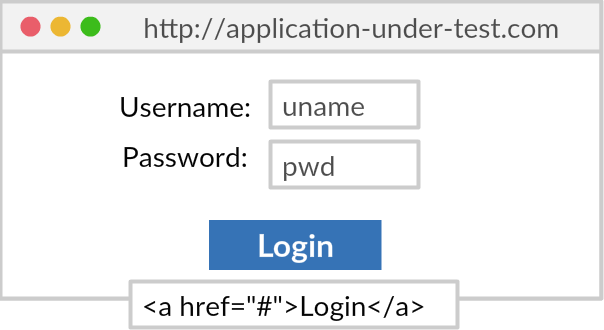
\includegraphics[width=5.6cm,height=2.8cm]{./Figures/newlogin}}
\vspace{-2mm}\subfigure[AUT version $V_{1}$]{\label{fig:b}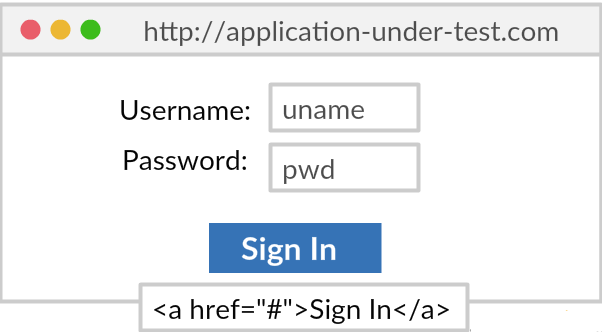
\includegraphics[width=5.6cm,height=2.8cm]{./Figures/newsignin}}
\caption{Visual comparison of version $V_{0}$ and $V_{1}$ of AUT}
\label{fig:loginTest}
\end{figure} 
% \begin{minipage}{0.45\textwidth}
% % \begin{figure}
% 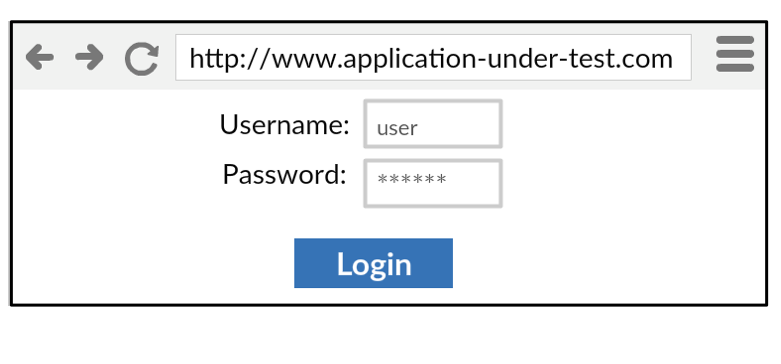
\includegraphics{./Figures/Login-button}
% \caption{Login}
% \label{fig:loginTest}
% % \end{figure}
% \end{minipage}%



% \begin{minipage}{0.5\textwidth}
% \begin{center}

% \begin{scriptsize}
% \lstset{
%   basicstyle=\ttfamily,
%   columns=fullflexible,
%   keepspaces=true,
% %   frame=none,
% }
% % \verb|basicstyle=\ttfamily, columns=fullflexible, keepspaces=true|
  
% \begin{lstlisting}[caption=Login test,label=code1]
% public void loginTest(){
% driver.get("http://www.application-under-test.com");
% driver.findElement(By.id("uname")).sendKeys("user");
% driver.findElement(By.id("pwd")).sendKeys("passwd");
% driver.findElement(By.linkText("Login")).click();
% }
% \end{lstlisting}
% \end{scriptsize} 
% \end{center}
% % \end{minipage}%

Compared to manual tests, Selenium tests can be run automatically and repeatedly. Typically, such tests can be combined with Continuous Integration tools to be run after the code changes are pushed to the version control repository. When AUT evolves from version $V_{0}$ to a newer version $V_{1}$, existing Selenium tests are executed on $V_{1}$. Ideally, if one or more tests executed successfully on $V_{0}$ fail to achieve the same result on $V_{1}$, the tests have found the possible \textit{software regressions} in the AUT. This approach in reality relies heavily on the quality and robustness of the existing tests. Intuitively, robustness of Selenium tests implies their reliability and effectiveness to achieve the same functional coverage across different versions of the AUT. 

% """However, as the web application continues to evolve, robustness of Selenium tests decreases over time."""

As the web application continues to evolve, existing Selenium tests might not achieve the same functional coverage as they do for the version the tests are originally written for. Consider the aforementioned example of \texttt{loginTest} where the outcome of code changes in AUT results in changing the display text of \textit{`Login'} button to ``Sign In'' in version $V_{1}$. When \texttt{loginTest} is re-run on $V_{1}$, it is unable to locate the \textit{`Login'} button since the hyperlink text ``Login'' is changed to ``Sign in''. As a result, \texttt{loginTest} is broken and the desired functional coverage is not achieved -- unless this fragile (non-robust) test is repaired. If Selenium tests are not robust and resilient enough as the AUT evolves, desired functional coverage is not achieved and regression testing becomes inefficient.


Unfortunately, such situations are not uncommon in agile development environments which involve frequent changes in the AUT \cite{martin2003agile}. The reasons for decreasing robustness and failures of Selenium tests includes changed functionality, modified GUI element locators, changed structural markup and timing issues etc. To repair the fragile tests, developers need to invest time and efforts to analyze the functionality changes, identify test failures manually and maintain such test-suites. In other words, when the AUT changes frequently, fragile tests need to be repaired repeatedly to cope with these changes, which can be an expensive and time consuming task for developers. 

As Selenium tests directly depend upon GUI element locators for locating desired object (e.g. a button) in the AUT, selection strategy for locating GUI elements plays vital role in dictating the robustness of Selenium tests. If a test implements structure based locators such as layout-dependent \texttt{xpath} expressions to find relative position of an element on the web page, slight changes in the structure of the web page can diminish the robustness of the test. Such situations can arise upon renaming the display hyperlink text (Figure \ref{fig:b}) or changing the HTML structure, such as changing the structure of the page through \texttt{<div>} tags. On the contrary, element locators such as unique element \texttt{id} attributes are not affected by such changes and can be used to write robust tests. 

Leotta et al. \cite{leotta2015using} present an algorithm for selecting reliable \texttt{xpath} locators from a set of absolute and relative \texttt{xpath} expressions for the AUT. Another study by Leotta et al. \cite{leotta2013comparing} compares the effort required to maintain \texttt{id, xpath} and \texttt{link text} locators. Nevertheless, these approaches cover only a subset of available element locators and measure the stability of Selenium tests in terms of the effort required to maintain these locators. Apart from the GUI element locators, the design and composition of tests such as the number of actions performed by the tests, mechanisms implemented to deal with timing issues (e.g.\smallskip implementing \texttt{wait} commands) also dictate the robustness of Selenium tests. 

% Robustness of Selenium tests can be defined in terms of their stability and effectiveness to achieve the same functional coverage across different versions of the AUT. 
% The reasons for decreasing robustness and failures of Selenium tests can include changed functionality, modified GUI element locators and changed structural markup, timing issues etc. 
% Such non-robust tests exhibiting decreased functional coverage are unsuitable for regression testing unless these tests are repaired. In order to modify such tests, developers need to invest time and efforts to analyze the undesired functionality changes, identify test failures manually and maintain such test-suites.

% In other words, if the Selenium tests are not robust enough, the regression testing is likely to be ineffective.

Considering the current state-of-the-art technologies to the best of my knowledge, thus far there has been no direct research in the area of assessing the robustness of Selenium tests over the version history of the web applications. Such analysis would help developers to understand the common reasons behind varying robustness of Selenium regression tests and write more robust tests. The primary goal of this thesis is to measure the robustness of Selenium test-suites over the version history of web applications and identify the factors affecting robustness. 

% \begin{figure}
% \begin{subfigure}[b]{0.31\textwidth} 
% 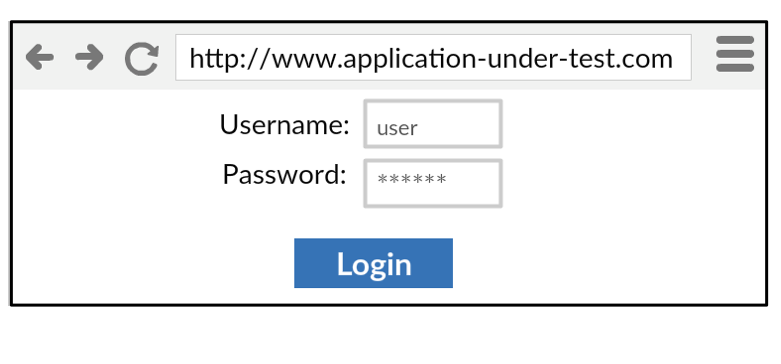
\includegraphics[width=7cm, height=3.2cm]{./Figures/Login-button}
% \caption{First subfigure}\label{fig:1a}
% \end{subfigure}
% \hspace*{\fill} % separation between the subfigures
% \begin{subfigure}{0.31\textwidth}
% 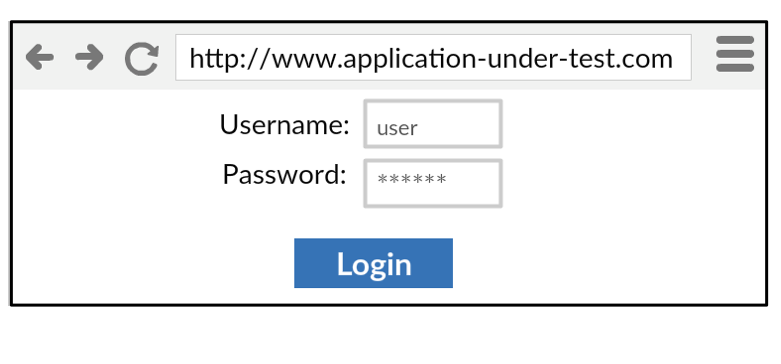
\includegraphics[width=7cm, height=3.2cm]{./Figures/Login-button}
% \caption{Second subfigure}\label{fig:1b}
% \end{subfigure}
% \caption{A figure that contains three subfigures}\label{fig:1}
% \end{figure}

% \subcaptionbox{The left subfigure with a long caption spanning several lines and some more text}%
%   [.4\linewidth]{\includegraphics[height=2cm]{example-image-a}}
%% THIS ONE WORKS !!!!!

% \begin{figure}
% 	\centering	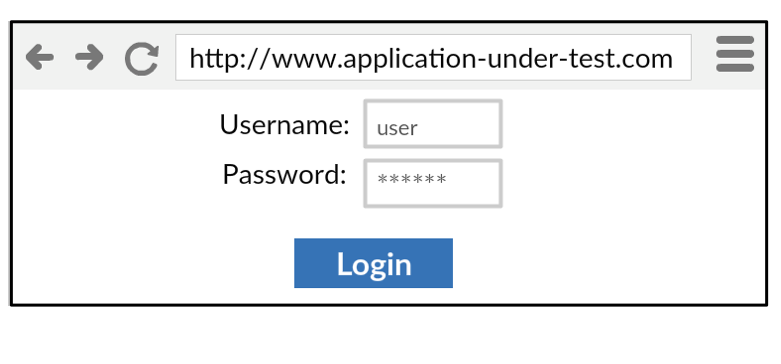
\includegraphics [width=7cm, height=3.2cm]{./Figures/Login-button}
% 	\caption{Login functionality of AUT}
% 	\label{fig:loginTest}
% \end{figure} 


The first step is to formally establish and define \textit{robustness} in terms of a measurable metric. A test can be marked as ``passed'' in the output logs but still land on different web pages of the AUT. Such test might not have covered the same functionality and cannot be considered robust. Furthermore, to identify the factors behind the varying robustness of Selenium tests, as mentioned earlier, a set of metrics have been developed. 

This thesis proposes the metric \textit{`robustness grade'} of a test which allows us to determine its effectiveness for regression testing. On a coarser level, \textit{`robustness grade'} of a test-suite can indicate its overall quality and suitability for regression testing. A high robustness can be another indication of the maintainability of the test-suite, since robust tests do not need to be repaired and maintained as frequently. If the proposed metrics are able to determine which factors impact robustness the most, developers can use these metrics to write more robust tests. This research aims to answer the following research questions:
\newline
{\bfseries RQ1} How robust are selenium tests against changes of the application under test? \newline
{\bfseries RQ2} Is robustness correlated to the design and composition of the tests?\newline
{\bfseries RQ3} Does the design of the test-suite influence the maintenance effort?\newline
{\bfseries RQ4} Can the robustness analysis improve current Selenium testing practices?\newline

% \\
% {\bfseries RQ1} How to determine the robustness of Selenium tests?
% {\bfseries RQ2} Is the change in robustness correlated to the changes of application’s structural elements?
% {\bfseries RQ4} Do tests with shorter execution traces tend to be more robust than tests with relatively longer traces?
% {\bfseries RQ5} Does same test input result in different GUI states of the AUT for different versions (\textit{reachability problem})?
% {\bfseries RQ6} Can the robustness analysis improve or assist current Selenium testing practices?
% {\bfseries RQ7} Reasons of failure behind test cases?
% {\bfseries RQ8} Size and complexity of test suite?
% \\

Figure \ref{fig:thesisoverview} depicts the setup required for performing the robustness analysis and answer aforementioned research questions. 
The first step is to select suitable testing candidates for this research and extract Selenium tests-suites from their test repositories. The approach is to deploy different versions of test candidates AUT and run automated Selenium regression tests on them. In the next step, Selenium tests are leveraged with the existing tool \texttt{webmate} \cite{webmate} to capture the application behavior in terms of behavioral state models. The \textit{states} of the state model represent the abstracted DOM (Document Object Model) states and \textit{transitions} represent actions executed on AUT. Such a state model allows us to compare the outcome of Selenium tests on different releases in comparison to the release for which the test-suite is written for. This step is essential for evaluating the functional behavior covered by the tests across different releases. Afterwards, \textit{`robustness grade'} is calculated for each test along with other metrics as defined in Chapter \ref{Chapter3}.\newline

\begin{figure}[h]
% [htbp]
	\centering	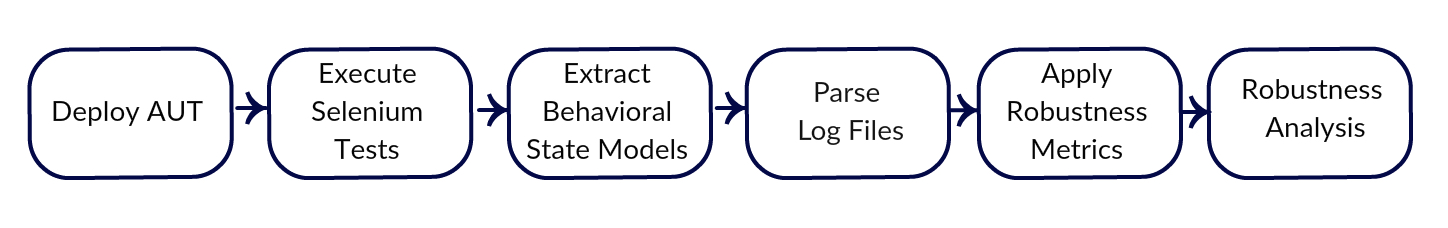
\includegraphics[width=\textwidth]{./Figures/thesisoverviewsmall.jpg}
%     [width=5cm, height=3cm]
% 		\rule{35em}{0.5pt}
	\caption{Setup required for the robustness analysis}
	\label{fig:thesisoverview}
\end{figure} 

This thesis is structured in following manner: Chapter 2 discusses the background terminologies. Chapter 3 discusses the approach for answering research questions. Chapter 4 provides the necessary implementation details of our approach. Chapter 5 presents the results and the evaluation of our approach. Chapter 5 discusses threats to validity. Chapter 6 discusses conclusion and future work. 
% \texttt{This section needs to be re-written}\newline
% \noindent This thesis is structured in following manner:
% \begin{itemize}
% \item Chapter 2 discusses the background terminologies
% \item Chapter 3 discusses the research questions in detail and provides necessary implementation details
% \item Chapter 4 presents the evaluation
% Approach and Evaluation : 20 pages
% Approach: Candidate selection, deployment, modifying selenium tests to fit to remotewebdriver, using sessionIDs to track, explaining how the entire grid works, extraction of state-models, comparison of GUI sequences, major minor versions,
% Evaluation: Experimental setup, test results, robustness metrics calculation, graphs, results
% For evaluating the approach and answer the research questions, the idea was to assess publicly available Selenium tests, in order to eliminate the possible bias introduced by writing one’s own Selenium tests as such are written from a single person’s design approach. In the same spirit, the presented model is tested on six different open source projects, from different domains as follows.
% \item Chapter 5 discusses threats to validity 
% \item Chapter 6 discusses conclusion and future work 
% \end{itemize}

